  The distance between two points is given by equation
 \begin{align}
 \brak{\vec{P}-\vec{Q}}^T\brak{\vec{P}-\vec{Q}}=10^2\\
\implies  \norm{P}^2 - \vec{P}^T\vec{Q} - \vec{Q}^T\vec{P} + \norm{Q}^2 = 100
 \end{align}
which, upon subsituting the values yields
 \begin{align}
 y^2 + 6y -27 &= 0\\
 \brak{y+9}\brak{y-3} &= 0
\implies y &= -9, 3
 \end{align}
and
\begin{align}
\vec{Q} = \myvec{10 \\3}, \myvec{10 \\-9}
\end{align}
 The python code to find the roots of the quadratic equation can be downloaded from
\begin{lstlisting}
solutions/7/codes/line/point_vec/roots.py
\end{lstlisting}
 The python code for Fig. \ref{fig:3.5.7}
can be downloaded from
\begin{lstlisting}
solutions/7/codes/line/point_vec/point_vec.py
\end{lstlisting}

\begin{figure}[!ht]
\centering
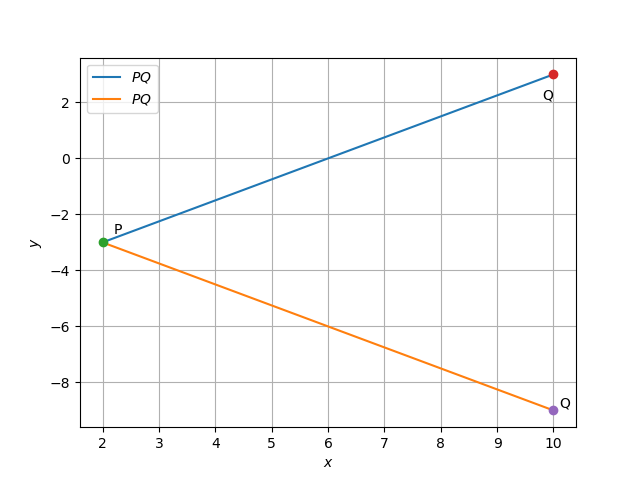
\includegraphics[width= \columnwidth]{./solutions/7/figs/line/point_vec/point_vec.eps}
\caption{}
\label{fig:3.5.7}
\end{figure}
 
